\documentclass[11pt,a4paper]{article}

\usepackage[utf8]{inputenc}
\usepackage[T1]{fontenc}
\usepackage{lmodern}
\usepackage[margin=2.5cm]{geometry}
\usepackage{amsmath,amssymb}
\usepackage{bm}
\usepackage{graphicx}
\usepackage{booktabs}
\usepackage{caption}
\usepackage{subcaption}
\usepackage{xcolor}
\usepackage[colorlinks=true,allcolors=blue!50!black]{hyperref}

\captionsetup{font=small,labelfont=bf}
\setlength{\emergencystretch}{2em}
\renewcommand{\UrlBreaks}{\do\/\do-\do.}

\newcommand{\F}{\bm{F}}
\newcommand{\PK}{\bm{P}}
\newcommand{\uu}{\bm{u}}
\newcommand{\vv}{\bm{v}}
\newcommand{\dd}{\,\mathrm{d}}

\title{Viscous polyconvex model:\\ calibration and numerical example}
\author{}
\date{Draft for co-authors --- \today}

\begin{document}
\maketitle

% =====================================================================
\section{Calibration}\label{sec:calibration}
% =====================================================================

\paragraph{Experimental data.}
The model is calibrated against the uniaxial tests on VHB 4910 reported in~\cite{Hossain2012}, digitised with~\cite{WPD}. Two datasets are used:
(i)~two quasi-static loading curves up to $\lambda=5$ (22 points), which characterise the equilibrium response, and
(ii)~eleven single loading--unloading cycles at constant stretch rates $\dot\lambda\in\{0.01,0.03,0.05\}\,\mathrm{s^{-1}}$ and maximum stretches $\lambda_{\max}\in\{1.5,2.0,2.5,3.0\}$ (1158 points), with test durations between 17\,s and 357\,s.

\paragraph{Model and test kinematics.}
The generalised Maxwell model combines a neo-Hookean equilibrium term, with shear modulus $\mu_e$, and $n$ viscous polyconvex branches, each characterised by a shear modulus $\mu_i$ and a relaxation time $\tau_i$.
Every test is reproduced at a single material point under homogeneous incompressible uniaxial tension, $\F=\mathrm{diag}(\lambda,\lambda^{-1/2},\lambda^{-1/2})$, with the hydrostatic pressure fixed by the traction-free lateral faces; the predicted nominal stress $P_{11}$ is compared with the measured one.
The internal variables are integrated with the time step $\Delta t=\Delta\lambda/\dot\lambda$ dictated by the stretch rate, using the \emph{same} constitutive routines and return mapping (HyperFEM) as the finite element simulation of Section~\ref{sec:example}. No constitutive law is re-implemented between calibration and simulation.

\paragraph{Two-step identification.}
The parameters minimise the normalised mean squared error over the $M$ curves of each dataset,
\begin{equation}
  \mathcal{L}(\bm{p}) = \frac{1}{M}\sum_{k=1}^{M}\frac{1}{N_k}\sum_{j=1}^{N_k}
  \left(\frac{P^{\mathrm{exp}}_{k,j}-P_{k,j}(\bm{p})}{\max_j |P^{\mathrm{exp}}_{k,j}|}\right)^2,
\end{equation}
in two sequential steps:
\textbf{Step 1}, $\mu_e$ is fitted to the quasi-static curves (Nelder--Mead);
\textbf{Step 2}, with $\mu_e$ fixed, the branch parameters $\{\mu_i,\tau_i\}_{i=1}^{n}$ are fitted simultaneously to the eleven cycles with a gradient-free, global particle swarm optimiser~\cite{Optim}.

\paragraph{Uncertainty.}
With the residual Jacobian $\bm{J}=\partial\bm{r}/\partial\bm{p}$ (central differences), the parameter covariance is estimated by the cluster-robust (sandwich) estimator~\cite{Cameron2015}
\begin{equation}
  \bm{\Sigma} = \frac{M}{M-1}\,(\bm{J}^{T}\bm{J})^{-1}\Big(\sum_{k=1}^{M}\bm{J}_k^{T}\bm{r}_k\bm{r}_k^{T}\bm{J}_k\Big)(\bm{J}^{T}\bm{J})^{-1},
\end{equation}
where residuals are clustered by experimental curve to account for their correlation along each curve.
Table~\ref{tab:calibration} reports the half-width of the 95\% confidence interval (margin), the relative error (margin/estimate) and the normalised sensitivity $S_j=2(\bm{J}^T\bm{J})_{jj}\,p_j^2/\mathrm{SSE}$, such that a relative perturbation $\varepsilon$ of $p_j$ increases the sum of squared errors by a factor $1+\tfrac12 S_j\varepsilon^2$.

\begin{table}[ht]
  \centering
  \caption{Calibrated parameters of VHB 4910 (two-branch model). Coefficients of determination: $R^2=0.995$ (step~1) and $R^2=0.977$ (step~2).}
  \label{tab:calibration}
  \begin{tabular}{l c r r}
    \toprule
    Parameter & Estimate $\pm$ margin (95\%) & Rel.\ error [\%] & Sensitivity \\
    \midrule
    \multicolumn{4}{l}{\textit{Step 1: Equilibrium term (neo-Hookean)}} \\
    $\mu_e$ [kPa]  & $13.4 \pm 0.24$ &  1.8 & 1278.6 \\
    \midrule
    \multicolumn{4}{l}{\textit{Step 2: Non-equilibrium terms (neo-Hookean branches)}} \\
    $\mu_1$ [kPa]  & $31.2 \pm 3.4$  & 11.0 & 18.0 \\
    $\tau_1$ [s]   & $6.45 \pm 1.9$  & 29.0 & 12.1 \\
    $\mu_2$ [kPa]  & $11.6 \pm 3.2$  & 27.5 & 48.1 \\
    $\tau_2$ [s]   & $140 \pm 76$    & 54.2 &  6.0 \\
    \bottomrule
  \end{tabular}
  % NOTE: values from README.md. Re-running Calibration.jl with HyperCalibration v0.0.3 gives
  %   mu_e = 13.4 +/- 0.092 kPa (0.7 %), and the simulation script uses tau_2 = 144.1 s.
\end{table}

\paragraph{Results.}
Two branches with well separated relaxation times, $\tau_1\approx6.5$\,s and $\tau_2\approx140$\,s, cover the time window of the experiments (Table~\ref{tab:calibration}).
Figure~\ref{fig:calibration} shows that the model captures the rate dependence, the hysteresis and the residual stretch after unloading, both across loading rates and across stretch amplitudes. The largest deviation, about 10\% of the peak stress at $\lambda_{\max}=2.5$, is attributable to the neo-Hookean equilibrium term, deliberately kept to limit the model to five parameters.

\begin{figure}[ht]
  \centering
  \begin{subfigure}[t]{0.49\textwidth}\centering
    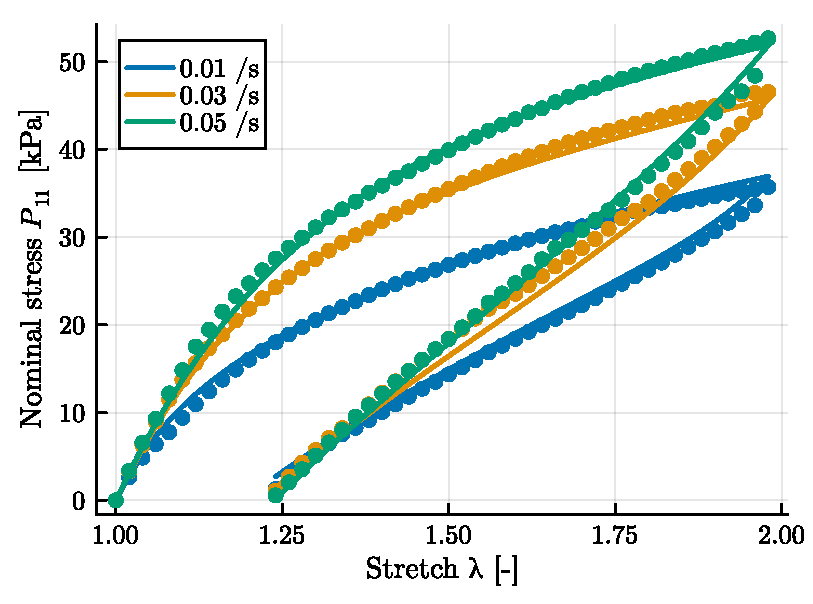
\includegraphics[width=\linewidth]{figures/calibration_fixed_stretch.pdf}
    \caption{$\lambda_{\max}=2.0$; $\dot\lambda=0.01,\,0.03,\,0.05\,\mathrm{s^{-1}}$.}
  \end{subfigure}\hfill
  \begin{subfigure}[t]{0.49\textwidth}\centering
    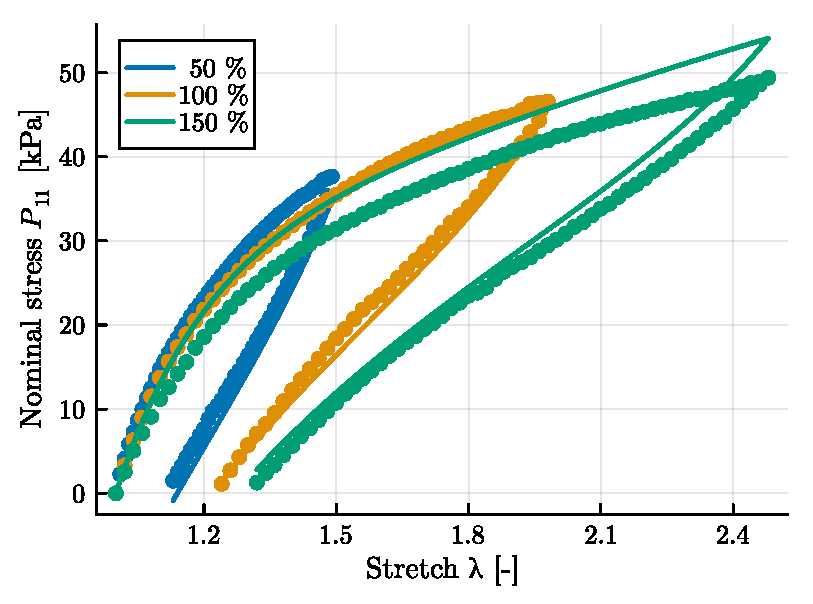
\includegraphics[width=\linewidth]{figures/calibration_fixed_rate.pdf}
    \caption{$\dot\lambda=0.03\,\mathrm{s^{-1}}$; $\lambda_{\max}=1.5,\,2.0,\,2.5$.}
  \end{subfigure}
  \caption{Calibrated model (lines) versus experimental data~\cite{Hossain2012} (markers) for uniaxial loading--unloading cycles of VHB 4910.}
  \label{fig:calibration}
\end{figure}

\paragraph{Number of branches.}
Figure~\ref{fig:uncertainty} propagates the parameter uncertainty to the predicted response: 100 parameter sets are sampled from $\mathcal{N}(\bm{p}^*,\bm{\Sigma})$ and evaluated on the test at $\lambda_{\max}=2.0$ and $\dot\lambda=0.03\,\mathrm{s^{-1}}$.
Adding a third branch leaves the fit unchanged ($R^2\approx0.977$ in both cases, loss reduction below 0.2\%), whereas the relative errors of the relaxation times grow from 29--54\% to above 400\%: the additional parameters are not identifiable from the available data. The two-branch model is therefore the richest one supported by the experiments, and it is the one used hereafter.
% NOTE: 3-branch figures from an unconstrained, seeded (Random.seed!(1234)) ParticleSwarm run: tau margins 438 % and 1180 %,
%   loss 2.2320e-3 vs 2.2345e-3 (2 branches). Update once the 3-branch figure is generated.

\begin{figure}[ht]
  \centering
  \begin{subfigure}[t]{0.49\textwidth}\centering
    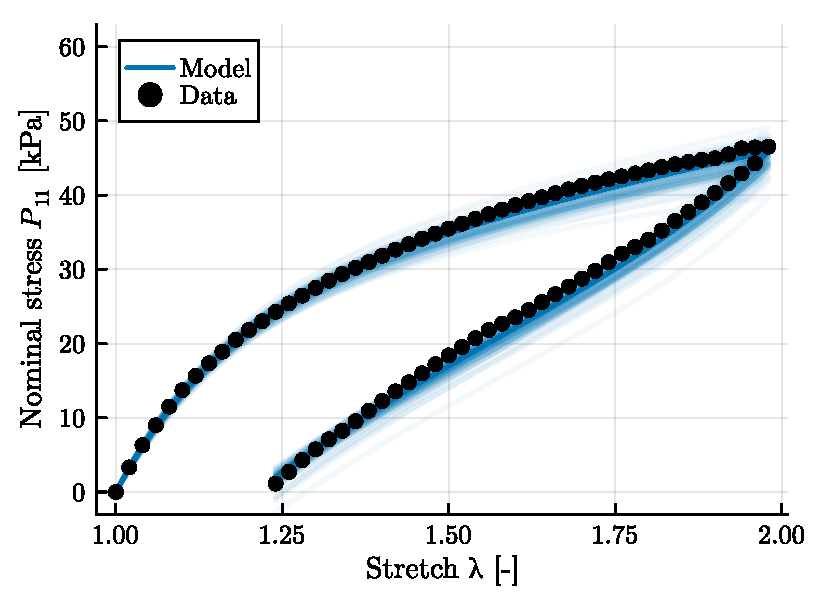
\includegraphics[width=\linewidth]{figures/uncertainty_2_branches.pdf}
    \caption{Two branches ($n_\textrm{Maxw}=2$).}
  \end{subfigure}\hfill
  \begin{subfigure}[t]{0.49\textwidth}\centering
    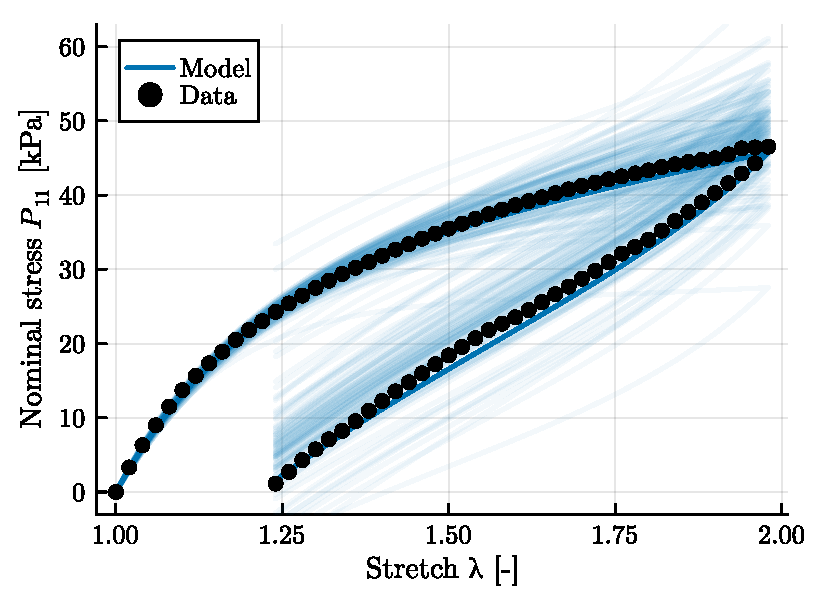
\includegraphics[width=\linewidth]{figures/uncertainty_3_branches.pdf}
    \caption{Three branches ($n_\textrm{Maxw}=3$).}
  \end{subfigure}
  \caption{Propagation of the parameter uncertainty (100 samples, shaded) for $\lambda_{\max}=2.0$ and $\dot\lambda=0.03\,\mathrm{s^{-1}}$; optimal model (solid line) and experimental data (markers).}
  \label{fig:uncertainty}
\end{figure}

\paragraph{Reproducibility.}
The whole section is produced by the script \texttt{calibration/Calibration.jl} of the repository~\cite{Repo} from the CSV data distributed with it, using HyperCalibration.jl~v0.0.3 and HyperFEM.jl~v0.0.6~\cite{HyperFEM}. It runs in about a minute on a laptop.

% =====================================================================
\section{Numerical example}\label{sec:example}
% =====================================================================

\paragraph{Problem set-up.}
A square membrane of side $w=200$\,mm and thickness $h=1$\,mm, $\Omega_0=(-w/2,w/2)^2\times(0,h)$, with density $\rho_0=960\,\mathrm{kg/m^3}$, is described by the two-branch model of Table~\ref{tab:calibration}, used as is. Near-incompressibility is enforced by the volumetric term $U(J)=\tfrac{\kappa}{2}(J-1)^2$ with $\kappa=2.5$\,MPa, i.e.\ $\kappa\approx45\,\mu_0$ with $\mu_0=\mu_e+\mu_1+\mu_2=56.2$\,kPa the instantaneous shear modulus; $|J-1|<6\cdot10^{-4}$ throughout the simulation.
No displacement constraint is prescribed (Figure~\ref{fig:setup}): the membrane is free-floating, so that no work is exchanged through reactions and the energy balance involves the applied load only.
The load is an out-of-plane traction $\bar{\bm{t}}=\bar t_0\,f(t)\,\bm{e}_3$, $\bar t_0=20$\,Pa, applied on the six faces of the central element, a $w/7\times w/7\times h$ block (peak resultant force $\approx35$\,mN). The pulse $f(t)$ is triangular: it grows linearly from 0 to 1 at $t=0.05$\,s and vanishes for $t\geq0.1$\,s, after which the membrane evolves freely.

\begin{figure}[ht]
  \centering
  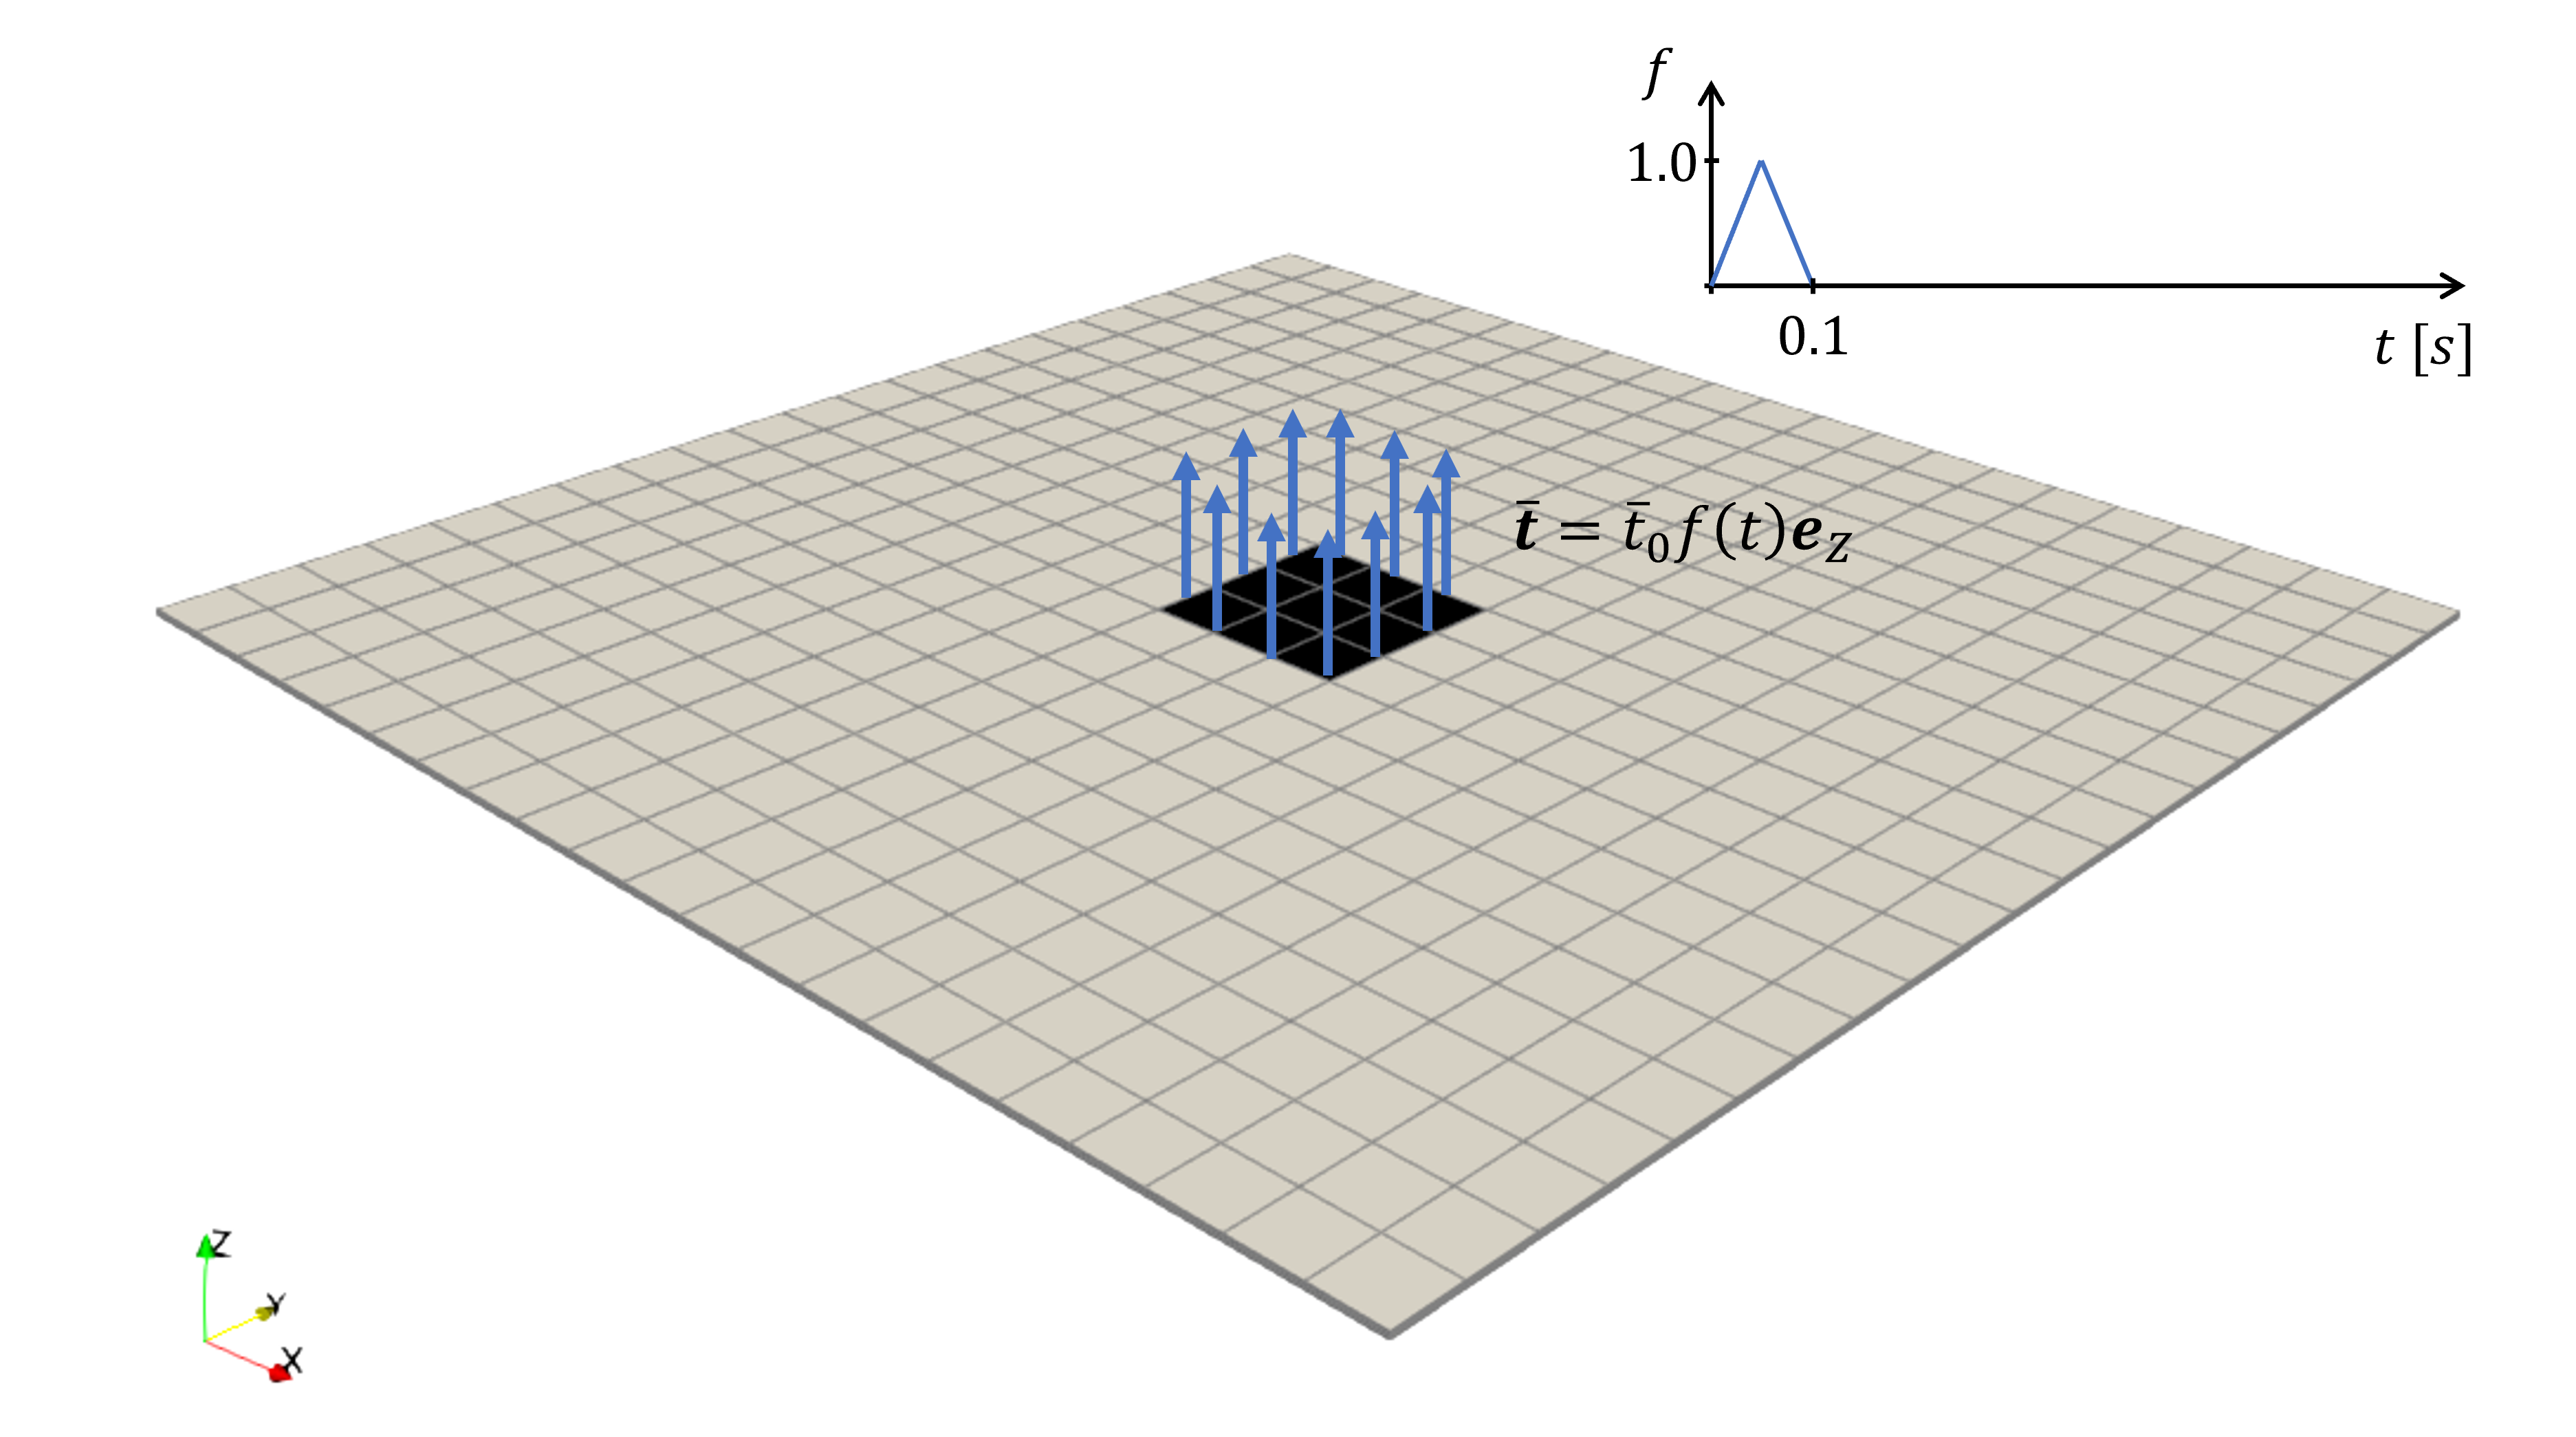
\includegraphics[width=\linewidth]{figures/membrane_setup.png}
  \caption{Free-floating square membrane: geometry, $7\times7\times1$ mesh, loaded central patch and time evolution $f(t)$ of the applied traction.}
  \label{fig:setup}
\end{figure}

\paragraph{Discretisation.}
The domain is discretised with $7\times7\times1$ hexahedra with triquadratic Lagrangian interpolation (2025 degrees of freedom) and Gauss quadrature exact for polynomials of degree~4.
Time integration is implicit with $\Delta t=1$\,ms up to $t=0.5$\,s (500 steps). With the velocity update $\tfrac12(\vv_{n}+\vv_{n+1})=(\uu_{n+1}-\uu_n)/\Delta t$, each step solves
\begin{equation}
  \int_{\Omega_0}\rho_0\,\frac{\vv_{n+1}-\vv_n}{\Delta t}\cdot\delta\uu\dd V
  +\int_{\Omega_0}\PK_{n+1/2}:\nabla_0\delta\uu\dd V
  =\int_{\Gamma_c}\bar{\bm{t}}(t_{n+1/2})\cdot\delta\uu\dd A,
\end{equation}
with $\PK_{n+1/2}=\tfrac12(\PK_n+\PK_{n+1})$, where $\PK_{n+1}=\partial_{\F}\Psi(\F_{n+1};\F_n,\mathcal{A}_n)$ is the algorithmic first Piola--Kirchhoff stress and $\mathcal{A}_n$ the internal variables of the branches, updated by the return mapping at the end of each step.
The nonlinear system is solved by Newton--Raphson with a direct solver (absolute and relative tolerances $10^{-8}$) within Gridap~\cite{Gridap}.

\paragraph{Energy balance.}
The kinetic energy $K$, the stored energy $\mathcal{E}$, the accumulated viscous dissipation $D$ and the external work $W_{\mathrm{ext}}$,
\begin{equation}
  \begin{gathered}
  K=\int_{\Omega_0}\tfrac12\rho_0|\vv|^2\dd V,\qquad
  \mathcal{E}=\int_{\Omega_0}\Psi(\F,\mathcal{A})\dd V,\\
  D=\int_0^t\!\!\int_{\Omega_0}\mathcal{D}\dd V\dd s,\qquad
  W_{\mathrm{ext}}=\sum_n\int_{\Gamma_c}\bar{\bm{t}}(t_{n+1/2})\cdot(\uu_{n+1}-\uu_n)\dd A,
  \end{gathered}
\end{equation}
are monitored at every step and must satisfy $K+\mathcal{E}+D=W_{\mathrm{ext}}$.
Figure~\ref{fig:energy} shows that the pulse injects $W_{\mathrm{ext}}=219\,\mu$J during $t\le0.1$\,s. Afterwards the membrane is isolated: energy is continuously exchanged between its kinetic and elastic parts, while the dissipation grows monotonically ($D=4.9\,\mu$J at $t=0.5$\,s). The balance residual $|K+\mathcal{E}+D-W_{\mathrm{ext}}|$ remains below $1.1\,\mu$J, i.e.\ below 0.5\% of the injected energy, over the 500 steps.

\begin{figure}[ht]
  \centering
  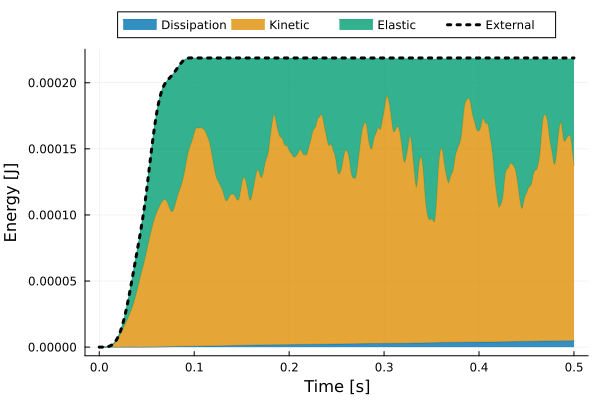
\includegraphics[width=0.75\linewidth]{figures/energy_balance.png}
  \caption{Energy balance: accumulated dissipation $D$, kinetic energy $K$ and stored energy $\mathcal{E}$ (stacked areas) versus the external work $W_{\mathrm{ext}}$ (dotted line).}
  \label{fig:energy}
\end{figure}

\paragraph{Deformation.}
Figure~\ref{fig:snapshots} shows the out-of-plane displacement at selected instants. The pulse bends the membrane around the loaded patch; the flexural wave reaches the free edges at $t\approx0.15$\,s, after which centre and edges oscillate in counter-phase. This motion is superposed on the rigid-body translation induced by the net impulse of the load (mean velocity $\approx4$\,cm/s).

\begin{figure}[ht]
  \centering
  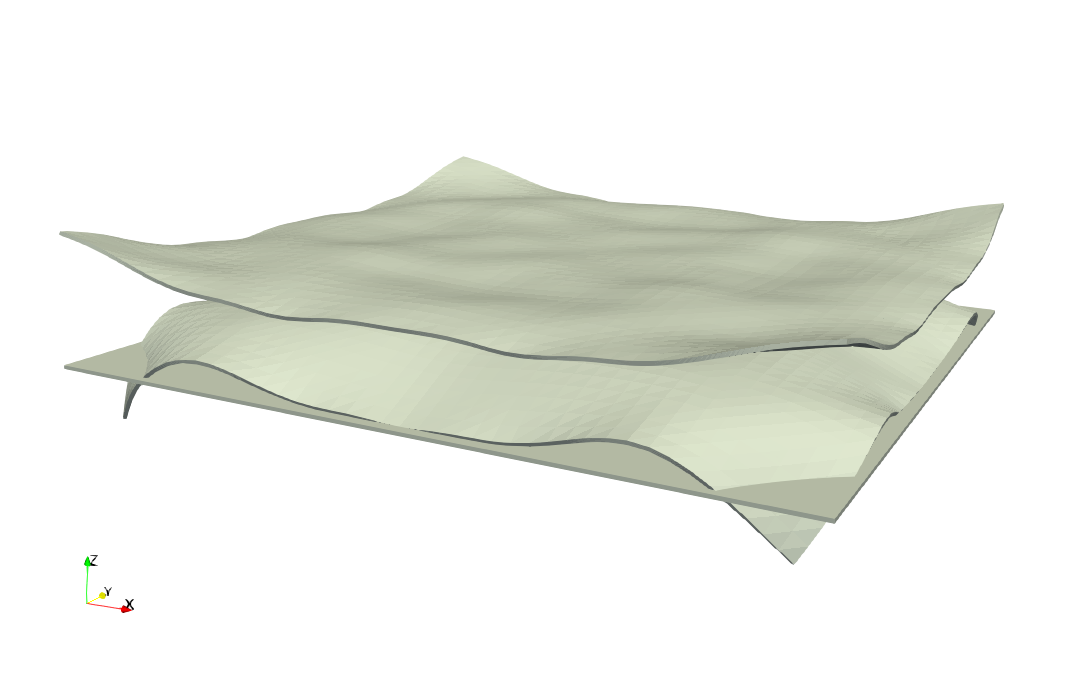
\includegraphics[width=\linewidth]{figures/mambrane_snapshots.png}
  \caption{Deformed configuration snapshots at $t=0\,,0.15$, and $0.3s$.}
  \label{fig:snapshots}
\end{figure}

{\sloppy
\paragraph{Reproducibility.}
The example is produced by the script \texttt{simulation/\allowbreak ViscoTimeIntegrator-\allowbreak Neumann.jl} of the repository~\cite{Repo}, with HyperFEM.jl~v0.0.6 and Gridap~v0.19. It writes the VTK snapshots and the energy history, and runs in about 5 minutes on a laptop; an independent re-run reproduces the energy history of Figure~\ref{fig:energy} exactly.\par}

% =====================================================================
\begin{thebibliography}{9}
\small
\bibitem{Hossain2012} M.~Hossain, D.~K.~Vu, P.~Steinmann, Experimental study and numerical modelling of VHB 4910 polymer, \emph{Comput.\ Mater.\ Sci.} 59 (2012) 65--74. \href{https://doi.org/10.1016/j.commatsci.2012.02.027}{doi:10.1016/j.commatsci.2012.02.027}.
\bibitem{WPD} A.~Rohatgi, WebPlotDigitizer v5.2, \url{https://automeris.io}.
\bibitem{Optim} P.~K.~Mogensen, A.~N.~Riseth, Optim: A mathematical optimization package for Julia, \emph{J.\ Open Source Softw.} 3 (24) (2018) 615.
\bibitem{Cameron2015} A.~C.~Cameron, D.~L.~Miller, A practitioner's guide to cluster-robust inference, \emph{J.\ Hum.\ Resour.} 50 (2) (2015) 317--372.
\bibitem{Gridap} F.~Verdugo, S.~Badia, The software design of Gridap: a finite element package based on the Julia JIT compiler, \emph{Comput.\ Phys.\ Commun.} 276 (2022) 108341.
\bibitem{HyperFEM} HyperFEM.jl, \url{https://github.com/MultiSimOLab/HyperFEM.jl}; HyperCalibration.jl, \url{https://github.com/miguelmaso/HyperCalibration.jl}.
\bibitem{Repo} \url{https://github.com/miguelmaso/2026-ViscousPolyconvex}.
\end{thebibliography}

\end{document}
